\documentclass[a4paper, 11pt, landscape]{article}

\usepackage{mathptmx} % more compact font
\usepackage{amsmath}
\usepackage{amsfonts}
\usepackage{mathtools}
\usepackage{multicol}
\usepackage{enumitem}
\usepackage{paralist} % for compacter lists
\usepackage{hyperref} % for Todo's and similar things
\usepackage[left=4.5mm, right=4.5mm, top=4.5mm, bottom=6mm, landscape, nohead, nofoot]{geometry}
\usepackage[small,compact]{titlesec}
\usepackage[extreme]{savetrees}
\usepackage[usenames,dvipsnames,svgnames,table]{xcolor}
\usepackage{xparse}
\usepackage{graphicx}
\usepackage{cancel}
\usepackage{dsfont}

% reinstate the Computer Modern calligraphic letters
\DeclareMathAlphabet{\mathcal}{OMS}{cmsy}{m}{n}
% change font
%\renewcommand{\familydefault}{\sfdefault}

% compact text
\linespread{0.9}
\setlength{\parindent}{0pt}

% compact lists even more
\setdefaultleftmargin{0em}{0em}{0em}{0em}{0em}{0em}

% compact sections
\titlespacing*{\section}{0pt}{0em}{0em}
\titlespacing*{\subsection}{0pt}{0em}{0em}
\titlespacing*{\subsubsection}{0pt}{0em}{0em}

% coloured section headings for easier read
\titleformat{name=\section}[block]
{\sffamily}
{}
{0pt}
{\colorsection}
\newcommand{\colorsection}[1]{%
	\colorbox{green!10}{\parbox[t][0em]{\dimexpr\columnwidth-2\fboxsep}{\thesection\ #1}}}

\titleformat{name=\subsection}[block]
{\sffamily}
{}
{0pt}
{\subcolorsection}
\newcommand{\subcolorsection}[1]{%
	\colorbox{lime!10}{\parbox[t][0em]{\dimexpr\columnwidth-2\fboxsep}{\thesubsection\ #1}}}


\titleformat{name=\subsubsection}[block]
{\sffamily}
{}
{0pt}
{\subsubcolorsection}
\newcommand{\subsubcolorsection}[1]{%
	\colorbox{lime!10}{\parbox[t][0em]{\dimexpr\columnwidth-2\fboxsep}{\thesubsubsection\ #1}}}

% environment for multicols inside a list
\NewDocumentEnvironment{listcols}{O{2} O{0pt}}
{%
	\bgroup %
	\setlength{\multicolsep}{#2} %
	\begin{multicols*}{#1} %
	}
	{%
	\end{multicols*} %
	\egroup %
}

% multicols lines & spacing
\setlength{\columnsep}{0.2cm}
\setlength{\columnseprule}{0.2pt}

% No page numbers
\pagenumbering{gobble}

% math helpers
\DeclareMathOperator*{\argmin}{arg\,min}
\DeclareMathOperator*{\argmax}{arg\,max}

\newcommand{\uP}{\mathrm P}

\begin{document}
	\begin{multicols*}{3}
		
		\defaultleftmargin{}{}{}{} 
		\section{Probabilities}
		\begin{compactitem}[]
			\item[] Bayes: $\uP(A\mid B) \; = \; \frac {\uP(B\mid A) \cdot \uP(A)} {\uP(B)} = \frac{\uP(A\cap B)}{\uP(B)}$
			\item[] $\uP(A\cap B) = \uP(A|B)\uP(B) = \uP(B|A)\uP(A)$
			\item[] $\uP(A\cup B)=\uP(A)+\uP(B)-{{\uP(A\cap B)}}$
			\item[] Chain rule $\uP (X_{1},.,X_{n})=\uP(X_{1})\,\uP(X_{2}| X_{1})\,\uP(X_{3}| X_{1},X_{2}) \cdots \uP(X_{n} | X_{1},.,X_{n-1})$
			\item[] Marginalization: $ \uP(X=x)=\sum _{y}\uP(X=x,Y=y)=\sum _{y}\uP(X=x\mid Y=y)\uP(Y=y)$
			\item[] Conditional independence: $X$ \& $Y$ are c.\ ind.\ given $Z$: $\uP(X, Y| Z) = \uP(X|Z) \uP(Y|Z)$ if $\uP(Y|Z) > 0$ that is equivalent to $\uP(X|Z,Y) = \uP(X | Z)$
		\end{compactitem}
	
	
		\section{Bayes Network}
		\textbf{Naive Bayes approach:} Effects are conditionally independent given a cause.
		
		\textbf{Bayesian network $(G,P)$:} directed, acyclic graph and a set of conditional probability distributions (CPTs) $\uP(X_s| Pa_{X_{s}})$
		
		 $(G,P)$ defines the joint distribution $\mathrm {P} (X_{1:n}) = \prod_{i} P(X_i| Pa_{X_{i}})$  
		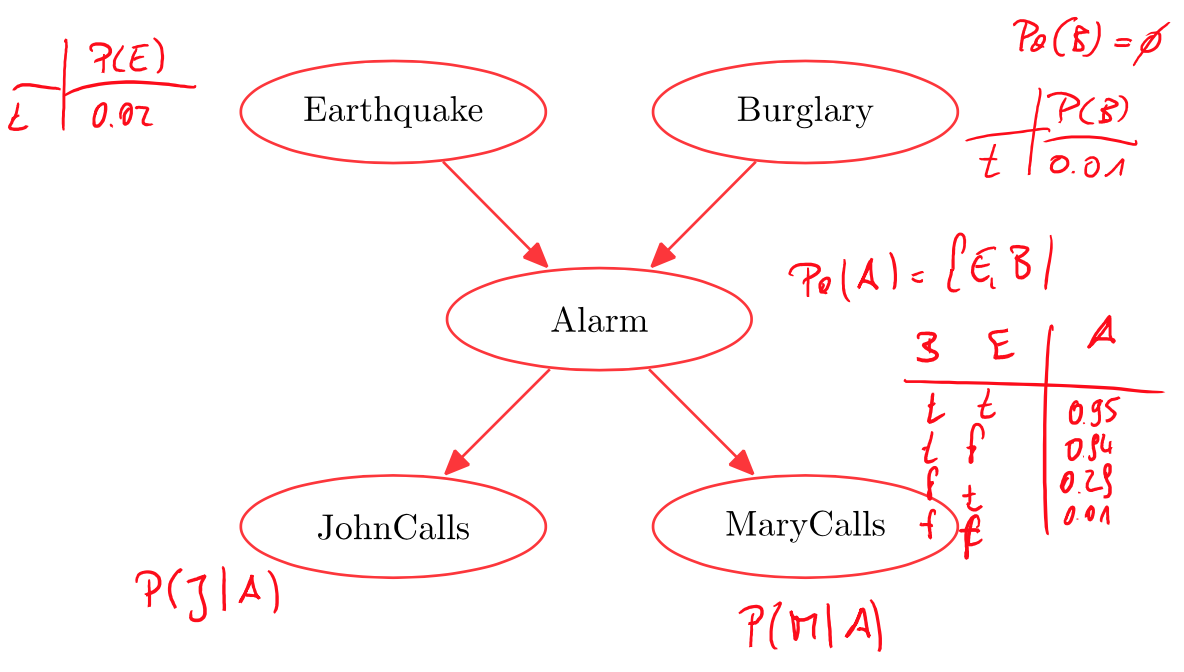
\includegraphics[height=2cm]{img/pai1.png}
		 
		\textbf{Specifying a BN}
		\begin{compactitem}
			\item Given random variables and known c. i.
			\item Pick ordering $X_1, \cdots, X_n$ of the variables
			\item For each $X_i$
			\begin{compactenum}
				\item Find minimal subset $A$ of $\{X_1,...,X_{i-1}\}$ such that $X_i \perp X_{\bar{A}} | X_A$ where $\bar{A} = \{1,...,i-1\}$ "minimal edges from existing variables to new variable in regards to c.i."
				\item Specify / learn $P(X_i|A)$
			\end{compactenum}
		\end{compactitem}
		BN defined this way are sound. Ordering matters a lot for compactness of representation!
		
		\textbf{Active Trails:}
		\begin{compactitem}
			\item  $X \rightarrow  Y \rightarrow Z$ \& $Y$ is unobserved
			\item  $X \leftarrow  Y \leftarrow Z$ \& $Y$ is unobserved
			\item  $X \leftarrow  Y \rightarrow Z$ \& $Y$ is unobserved
			\item  $X \rightarrow  Y \leftarrow Z$ \& $Y$ or any of $Y's$ descendants is oberserved
		\end{compactitem}
	
		Any variables $X$ and $Y$ for which there is no active trail for observations $Z$ are called d‐separated by $Z$. 
		
		$d$-$sep(X;Y | Z) \Rightarrow X \perp Y | Z$
		
		\section{Inference}
		\textbf{Typical Queries:} Conditional Distribution, MPE ($\argmax_{e,b,a} P(e,b,a | J=t, M = f)$), MAP ($\argmax_{e} P(e | J=t, M = f)$)
		
		\subsection{Exact Inference}
		
		\textbf{Variable Elimination}
		
		\begin{compactitem}
			
		\item Given BN and Query $P(Q | E=e)$ ($E$ = evidence variables)
		\item Choose an ordering of $X_1, ..., X_n$
		\item Set up initial factors: $fi = P(X_i | P_{ai})$
		\item For $i =1:n$, $X_i  \in X\setminus \{Q,E\}$
		\begin{compactenum}
			\item Collect and multiply all factors $f$ that include $X_i$  
			\item Generate new factor by marginalizing out $X_i$
			\item Add $g$ to set of factors, $g = \sum_{x_i}\prod_{j}f_j$
		\end{compactenum}
		\item  Renormalize $P(q,e)$ to get $P(q | e)$ = $\dfrac{1}{\sum_{q}P(q,e)}P(q,e)$
		
	\end{compactitem}
	
	\textbf{Example:} TODO
		
	\textbf{Variable Elimination for Polytrees}
	
	Polytree: A DAG is a polytree iff dropping edge directions results in a tree
	\begin{compactitem}
		\item Pick root
		\item Orient edges towards the root
		\item Eliminate in topological ordering (descendants for parents)
	\end{compactitem}

	Cutset Extension??
	
	\textbf{Factor Graphs}
	A factor graph for a BN is a bipartite graph with variables on one side and  factors on the other.
	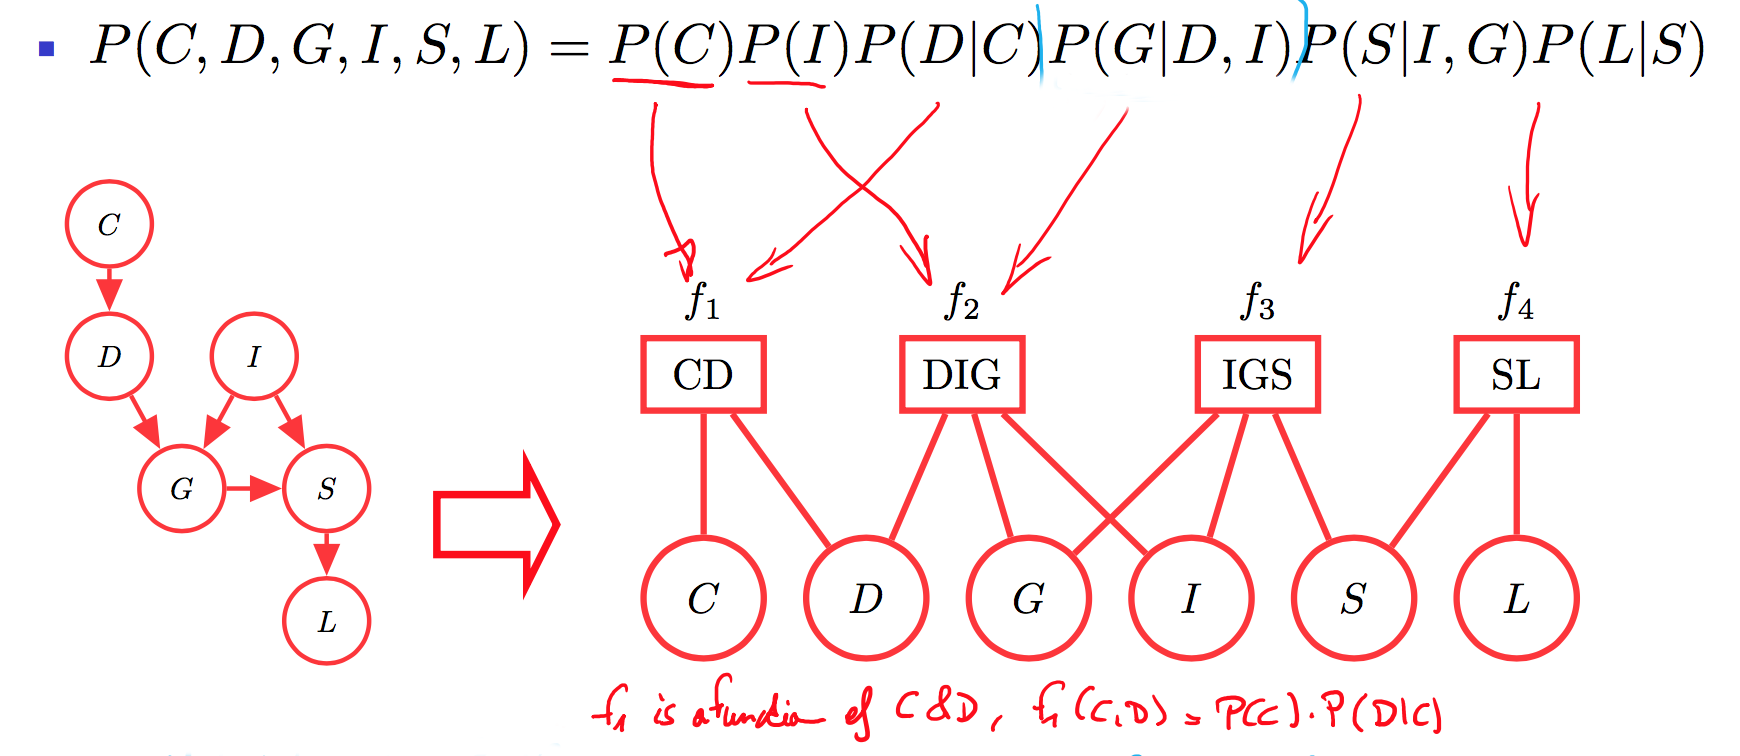
\includegraphics[height=2cm]{img/pai2.png}
	
	\textbf{Sum-Product / Belief Propagation Algorithm}	
	
	\begin{compactitem}
		\item Initialize all messages as uniform distribution  
		\item Until converged do
		\begin{compactenum}
			\item Pick some ordering on the factor graph edges (+directions)   
			\item Update messages according to this ordering
			
			Messages from variable v to factor u: 
			
			$\mu_{v \rightarrow u} = \prod_{u' \in N(v) \setminus \{u\}} \mu_{u' \rightarrow v}(x_{v})$ 
			
			Messages from factor u to variable v:
			
			$\mu_{u \rightarrow v} = \sum_{x_u \sim x_v} f_u(x_u) \prod_{v' \in N(u) \setminus \{v\}} \mu_{v' \rightarrow u}(x_{v'})$ 

			\item Break once all messages change by at most $\epsilon$
		\end{compactenum}
	\end{compactitem}

	\textbf{Example:} TODO

	\textbf{Belief Propagation on Trees}
	\begin{compactitem}
		\item Factor graph of polytree is a tree!
		\item Choose one node as root
		\item Send messages from leaves to root, and from root to leaves
	\end{compactitem}
   
\textbf{Variable Elimination for MPE}	
	\begin{compactitem}
	\item Given BN and evidence $E=e$
	\item Choose an ordering of $X_1, ...,X_n$
	\item Set up initial factors: $f_i = P(X_i | Pa_i)$
	\item For $i=1:n, X_i \notin  E$
  	\begin{compactenum}
  	\item Collect and multiply all factors $f_j$ that include $X_i$   
  	\item Generate new factor by maximizing out $X_i$
  	
	$g_i = \max_{x_i} \prod_{j} f_j$
  	\item Add $g$ to set of factors
  	\end{compactenum}
	\item For $i=n:-1:1, X_i \notin  E$:  $\hat{x_i} = \argmax_{x_i} g_i(x_i, \hat{x}_{i+1:n})$
\end{compactitem}

\textbf{Example: }

$\argmax_{e , b, a} P(e,b,a| J, M) = \argmax_{e , b, a} \bcancel{\frac{1}{Z}} P(e,b,a, J,M)$

$= \argmax_{e , b, a} P(e)P(b)P(a|e,b)P(J|a)P(M|a)$

$= \argmax_{a} P(J|a)P(M|a)  \argmax_{e} P(e)  \argmax_{b} P(b)P(a|e,b)$

$a^{*} = \argmax_{a} P(J|a)P(M|a) g_e(a)$

$e^{*} = \argmax_{e} P(J|a^*)P(M|a^*) P(e) g_b(a^*,e)$


\textbf{Max-product Message Passing on Factor Graphs}

Messages from variable v to factor u: 

$\mu_{v \rightarrow u} = \prod_{u' \in N(v) \setminus \{u\}} \mu_{u' \rightarrow v}(x_{v})$ 

Messages from factor u to variable v:

$\mu_{u \rightarrow v} = \max_{x_u \sim x_v} f_u(x_u) \prod_{v' \in N(u) \setminus \{v\}} \mu_{v' \rightarrow u}(x_{v'})$ 
 
 \textbf{Retrieving MAP From Max-Product}
 \begin{compactitem}
 \item Define max-marginals: $P_{max}(X_v =x_v) = \max_{x \sim x_v} P(x)$
 \item For tree factor graphs, max-product computes max-marginals: 
 $P_{max}(X_v = x_v) \propto \prod_{u \in N(v)} \mu_{u \rightarrow v} (x_v)$ 
\item Can retrieve MAP solution from these (must be careful when ties need to be broken)
\end{compactitem}
\subsection{Approximate Inference}
Problem: if BN contains loops.
Loopy belief propagation will in general not converge	$\rightarrow$ Sampling Based Inference

\textbf{Monte Carlo Sampling from a BN (forward Sampling)}
\begin{compactitem}
	\item Sort variables in topological ordering $X_1,...,X_n$
	\item For $i=1$ to 	$n$ do: Sample $xi \sim P(X_i | X_1=x_1, ..., X_{i-1}=x_{i-1})$
\end{compactitem}

\textbf{Computing Probabilities Through Sampling}

Marginals: $P(w=t) \approx \frac{1}{N} \sum_{i=1}^{N}[w=t](x^{(i)} =\frac{ Count(w=t)}{N}$

Conditionals: $P(C=t | W=t) = \frac{P(C=t, W=t)}{P(w=t)} \approx \frac{Count(W=t, C=t)}{Count(W=t)ß}$

\textbf{Rejection Sampling}
"Normaler Wuerfel nehmen um Verteilung von 1..5 zu samplen, 6 wir jeweils ignoriert"

$\hat{P}(X_A = x_A | X_B = x_B) \approx \frac{Count(x_a, x_B)}{Count(x_B)}$

Trow away samples that disagree with $x_B$, can be problematic if $x_B$ is a rare event. 

\textbf{Markov Chain}

A (stationary) Markov chain is a sequence of RVs, $X_1,...,X_N$ with Prior $P(X_1)$ \& transition probabilities $P(X_{t+1} | X_t)$ independent of $t$.


Ergodic: if there exists a finite $t$ such that every state can be reached from every state in exactly $t$ steps. Ergodic MC has a unique \& positive stationary distribution.

\textbf{Sampling from MC}
Sample $x_1~P(X_1)$, Sample $x_2~P(X_2 | X_1=x_1)$,..., Sample $x_N~P(X_N | X_{N-1}=x_{N-1})$.
If simulated “sufficiently long”, sample $X_N$ is drawn from a distribution “very close” to stationary distribution $\pi$.

\textbf{Markov Chain Monte Carlo (MCMC)}
TODO: Slide 6 P29- 32

\textbf{Gibbs Sampling: Random Order}
\begin{compactitem}
\item Start with initial assignment $x$ to all variables
\item Fix observed variables $X_B$ to their observed value $x_B$
\item For $t=1$ to $\infty$ do
\begin{compactenum}
\item Pick a variable $i$ uniformly at random from $\{1,..,n\} \setminus B$
\item Set $v_i = $values of all $x$ except $x_i$
\item Update $x_i$ by sampling from $P(X_i | v_i)$
\end{compactenum}
\end{compactitem}
Satisfies detailed balance equation!

\textbf{Gibbs Sampling: Practical Variant}
\begin{compactitem}
 \item Start with initial assignment $x^{(0)}$ to all variables
 \item Fix observed variables $X_B$ to their observed value $x_B$
 \item For $t=1$ to $\infty$ do 
\begin{compactenum}
\item Set $x^{(t)} = x^{(t-1)}$
\item For each variable $X_i$ (except those in $B$) 
\item Set $v_i =$ values of all $x^{(t)}$ except $x_i$
\item Sample $x_i^{(t)}$ from $P(X_i | v_i)$
\end{compactenum}
\end{compactitem}
No detailed balance, but also has correct stationary distribution.

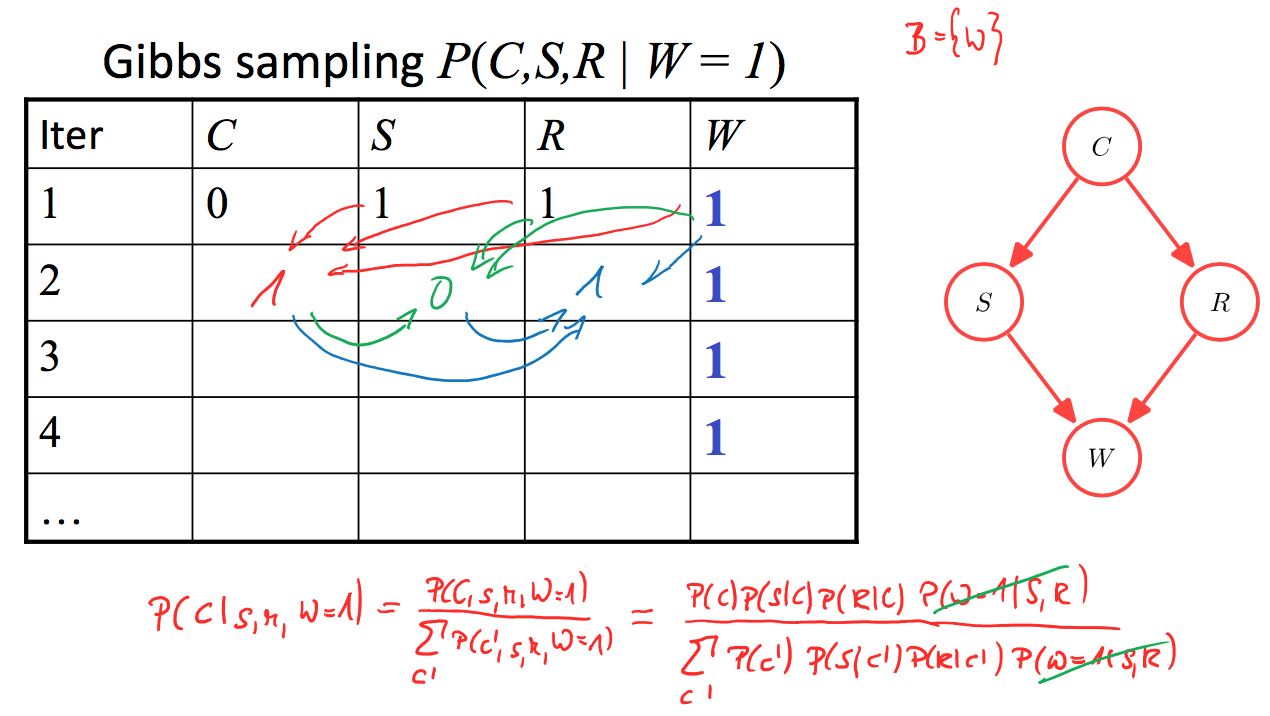
\includegraphics[height=2.5cm]{img/pai3.png}

\subsection{Temporal models}

\textbf{Markov Chains}

Markov assumption: $x_{t+1} \perp x_{1:t-1} | x_t \forall t$

Stationary asm.: $P(x_{t+1} = x | x_t = x') = P(x_{t'+1} | x_{t'} = x') \forall t, t'$

Order: 2nd-order next state depend on last two states, k-order last k states. 

\textbf{Prediction in Markov Chains}

$P(X_3 | X_1 = x) = \sum_{X_2}P(X_3,X_2|X_1 = x) = \sum_{X_2}P(X_3 | X_2, X_1 = x)P(X_2 | X_1 = x) =  \sum_{X_2}P(X_3 | X_2)P(X_2 | X_1 = x) = f(P(X_2|X_1))$

$P(X_4 | X_1 = x) = \sum_{X_3}P(X_4,X_3|X_1 = x) = \sum_{X_3}P(X_4 | X_3)P(X_3 | X_1 = x) = f(P(X_3|X_1)) = f(f(P(X_2 | X_1)))$

\textbf{Hidden Markov Model/ Kalman Filters}

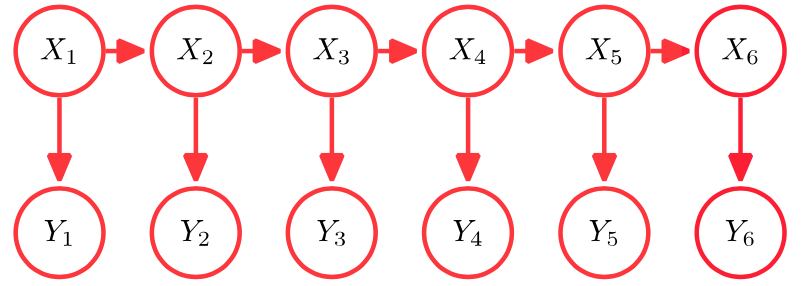
\includegraphics[height=1cm]{img/pai4.png}
$X_1,...,X_T$: Unobserved (hidden) variables (called states) \\
$Y_1,...,Y_T$: Observations \\
HMMs: $X_i$ categorical, $Y_i$ categorical (or arbitrary)\\
Kalman Filters: $X_i, Y_i$ Gaussian distributions

\textbf{Inference Tasks}

Filtering: $P(X_t | y_{1:t} ) $\\
Prediction: $P(X_{t+T} | y_{1:t} )$ \\
Smoothing: $P(X_t | y_{1:T}) \text{ for } 1\leq t < T$\\
MPE: $\argmax_{X_{1:T}} P(X_{1:T} | y_{1:T})$
 
In principle, can use variable elimination / belief propagation with new variables Xt, Yt at
each time step. Problem need to rerun every time, complexity grows with time!

\textbf{Bayesian Filtering}
Suppose we already have computed $P(X_t | y_{1,...,t})$ now want to efficiently compute $P(X_{t+1} | y_{1,...,t+1})$

\begin{compactitem}
	\item Start with $P(X_1)$
	\item At time $t$ (Assume we have:  $P(X_t | y_{1,...,t-1})$
	\item Conditioning: $P(X_t | y_{y1:t}) = \frac{1}{Z} P(X_t | y_{1:t-1})P(y_t | X_t)$
	\item $Z= \sum P(x,y_t | y_{1:t-1})$ ???
	\item Prediction: $P(X_{t+1} | y_{y1:t}) = \sum_{x_t}  P(X_t | y_{1:t}) P(X_{t+1} | x_t)$
\end{compactitem}
Computation is recursive (cost independent of t)!

\textbf{Kalman Filtering}
TODO: ???

\textbf{Dynamic Bayesian Networks}
If we have more than one variable at each time step
\begin{compactitem}
	\item At every timestep have a replicated BN
	\item Variables at each time step $t$ called a slice $S_t$
	\item “Temporal” edges connecting $S_{t+1}$ with $S_t$ (usually sharing parameters - stationarity)
	\item Can use standard approximate inference techniques (many loops) but high complexity over timesteps
\end{compactitem}


\textbf{Particle filtering}
Approximate the posterior at each time by samples (particles), which are propagated and reweighted over time.
True distribution (possibly continuous): $P(x)$, $N$ i.i.d. samples: $x_1,..x_N$; Represent: $P(x) \approx \frac{1}{N} \sum_{i=1}^{N} \delta_{x_i}(x)$

\begin{compactitem}
	\item Suppose $P(X_t | y_{1:t}) \approx \frac{1}{N} \sum_{i=1}^{N} \delta_{x_i, t}$
	\item Prediction: Propagate each particle: $x'_i \sim P(X_{t+1} | x_{i,t})$
	\item Conditioning: Weigh particles: $w_i = \frac{1}{Z}P(y_{t+1} | x'_i)$
	\item Conditioning: Resample $N$ particles: $x_{i, t+1} \sim \frac{1}{N} \sum_{i=1}^{N} w_i\delta_{x'_i}$ 
\end{compactitem}

\subsection{Probabilistic planning}
How should we control the robot to maximize reward?

\textbf{Markov Decision Processes (MDP)}
"controlled Markov chain", an MDP is specified by:
\begin{compactitem}
	\item A set of states $X={1,...,n}$
	\item A set of actions $A={1,...,m}$
	\item Transition probabilities $P(x’ | x, a)$ = Prob(Next state = $x’ |$ Action $a$ in state $x$)
	\item A reward function r(x, a)
	
	Modes: Finite horizon ($T timesteps$) or Discounted rewards (inf timesteps but discount future rewards)
\end{compactitem}

\textbf{Policy}
Deterministic (fixed) policy $\pi: X \rightarrow A$

Value of policy: 

$V^\pi(x)$ $= J(\pi | X_0 = x) $$= \mathds{E}[\sum_{t=0}^{\infty} \gamma^t r(X_t, \pi(X_t)) | X_0 = x] $

$= r(x, \pi(x)) + \gamma \sum_{x'} P(x' | x, \pi(x)) V^\pi(x')$

Can compute $V\pi$ exactly by solving linear system! 

\textbf{Value functions and policies}


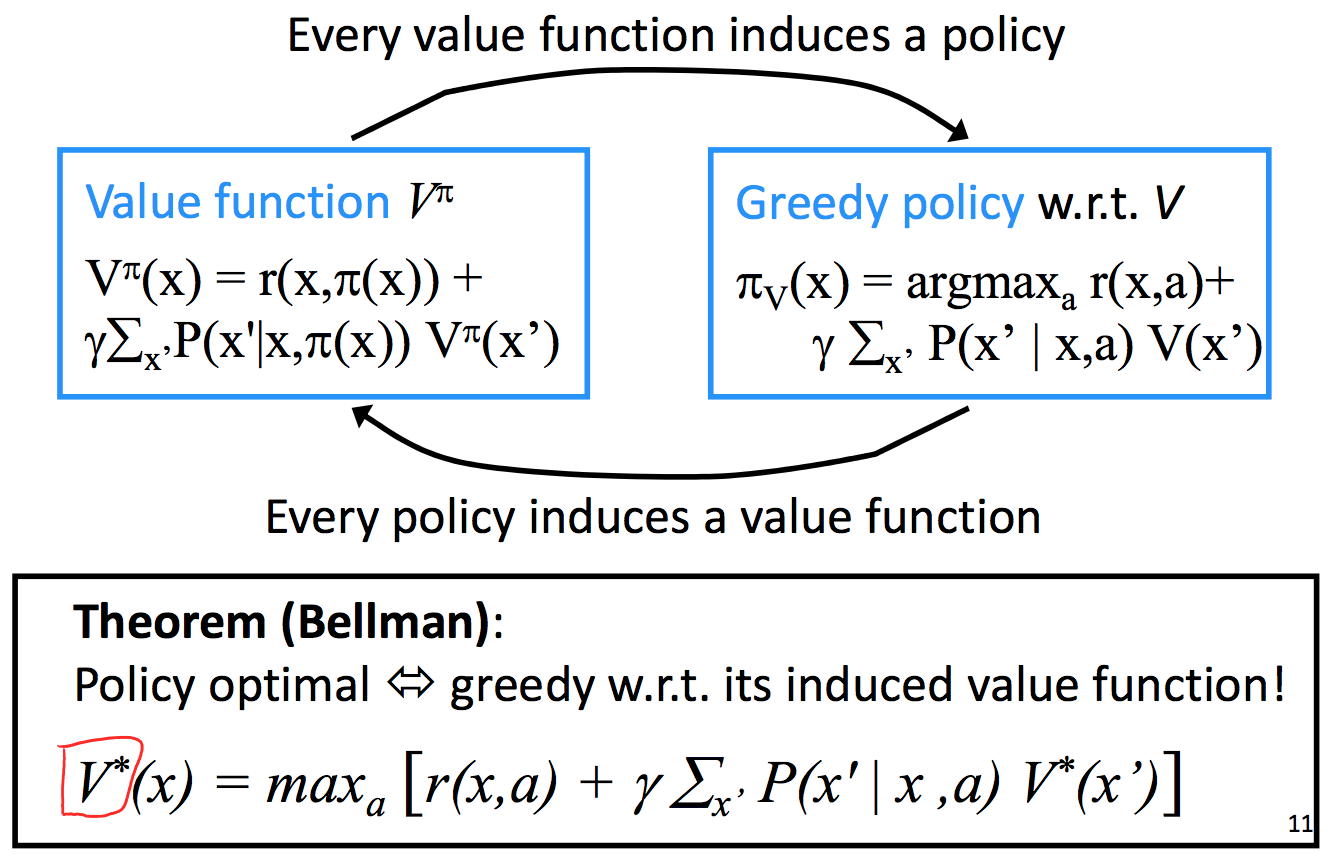
\includegraphics[height=3.5cm]{img/pai5.png}

\textbf{Policy iteration}
\begin{compactitem}
	\item Start with an arbitrary (e.g., random) policy $\pi$
	\item Until converged do:
	\item Compute value function $V^\pi(x)$
	\item Compute greedy policy $\pi_G$ w.r.t. $V^\pi$
	\item Set $\pi \leftarrow \pi_G$
\end{compactitem}

Guaranteed to monotonically improve \& converge to an optimal policy.

\textbf{Value iteration}
\begin{compactitem}
\item Initialize $V_0(x) = \max_a r(x, a)$
\item For $t=1$ to $\infty$ 
\item For each $x, a$, let $Q^t(x,a) = r(x, a) + \gamma \sum_{x'} P(x' | x, a) V^{t-1}(x'))$
\item For each x let $V^t(x) = \max_a Q^t(x,a)$
\item Break if $max_x V^t(x) - V^{t-1}(x) < \epsilon$
\item Then choose greedy policy w.r.t. $V_t$
\end{compactitem}

Guaranteed to converge to $\epsilon$-optimal policy!

\textbf{Tradeoffs: Value vs Policy Iteration}
Policy iteration: Finds exact solution in polynomial \# iterations. Complexity per iteration: $O(n^3)$
Value iteration: Finds ε-optimal solution in polynomial \# iterations. Complexity per iteration: $O(n\cdot m \cdot a)$

\textbf{Partially Observable MDP (POMDP)}

"controlled HMM"
Key idea: Interpret POMDP as an MDP with enlarged state space: New states correspond to beliefs $P(X_t | y_{1:t})$ in the original POMDP
TODO: Belief-state MDP / Policy gradient methods ??

\section{Learning BN}
Learn from i.i.d. data: 1.) Learning structure (conditional independencies) 2.) Learning parameters (CPDs)

\subsection{Parameter learning} 

$P(X_1, ..., X_N) = \prod_{i=1}^{n} P(X_i | Pa_i, {\theta}_{i | Pa_i})$

Given:  BN structure $G$ \& Data set $D$ of complete observations
For each variable $X_i$ estimate: $\hat{\theta}_{X_i | Pa_i} = \frac{Count(X_i , Pa_i)}{Count(Pa_i)}$ (MLE)

We can also use a Beta prior. (A priori knowledge)

\subsection{Structure learning}

Score based structure learning: scoring function S(G;D). Quantifies, for each structure G the fit to the data D. 

$G^* = \argmax_G S(G;D)$

Again use MLE: $S(G;D) = \max_\theta \log P(D | \theta, G)$
$\log P(D | \theta_{G (MLE for G)}) = N \sum_{i=1}^{n} \hat{I}(X_i ; Pa_i) + const$

Mutual Information: $I(X_i; X_j) = \sum_{x_i, x_j} P(x_i, x_j) \log \frac{P(x_i, x_j)}{P(x_i) P(x_j)}$
Empirical MI: 

$\hat{P}(x_i, x_j) = \frac{Count(x_i, x_j)}{N}; \hat{I} = \sum_{x_i, x_j} \hat{P}(x_i, x_j) \log \frac{\hat{P}(x_i, x_j)}{\hat{P}(x_i) \hat{P}(x_j)}$

Problem: Optimal solution for MLE is always the fully  connected graph. 

\textbf{Bayesian Information Criterion (BIC)}
(Regularizing) $S_{BIC}(G) = \sum_{i=1}^{n} \hat{I}(X_i ; Pa_i) - \frac{\log N}{2N} |G|$ where $|G|$ is \# of parameters of G, n is \# of variables, N is \# of training examples

Haha this is now NP hard but find optimal tree-shaped BN is possible

\textbf{Chow-Liu algorithm}
\begin{compactitem}
	\item For each pair $X_i, X_j$ of variables compute $\hat{P}(x_i, x_j)$
	\item Compute MI $\hat{I}(X_i, X_j)$
	\item Define complete graph with weight of edge $(X_i,X_j)$ given by the MI
	\item Find maximum spanning tree $\rightarrow$ undirected tree
	\item Pick any variable as root and orient the edges away using bfs

\end{compactitem}


\section{Reinforcement Learning}
"Learn mapping from (seq. of) actions to rewards"

\subsection{Passive Reinforcement}
Execute a set of trials in the environment using (fixed) policy  $\pi$
Reduction to a supervised problem. But does not exploit that values of states are not independent! (Bellman)

\subsection{Active Reinforcement Learning}
We are not interested in a fixed policy, but need to decide which action to take in every state. Fundamental Dilemma: Exploration-Exploitation Dilemma in RL

\begin{compactitem}
	\item Always pick a random action - will eventually estimate all prob and rewards. May do extremely poorly. 
	\item Always pick the best action according to current knowledge - quickly get some rewards but can get stuck in suboptimal action.
\end{compactitem}

\subsubsection{Model-based RL }
Learn the MDP - optimize policy based on MDP.

\textbf{Learning the MDP}

Estimate transitions: $\hat{P}(X_{t+1} | X_t, A_t) = \frac{Count(X_{t+1}, X_t, A_t)}{Count(X_t, A_t)}$

Estimate rewards: $\hat{r}(X=x, A= a) = \frac{\sum_{t: x_t = x, a_t = a} r_t}{Count(X = x, A = a)}$

\textbf{ $\epsilon_t$ greedy}
With probability  $\epsilon_t$: Pick random action; With probability $(1- \epsilon_t)$: Pick best action

\textbf{$R_{max}$ Algorithm}

If you don’t know $r(x, a)$ : set it to $R_{max}$

If you don’t know $P(x' | x, a)$: set $P(x^* | x, a) = 1$ where $x^*$ is a “fairy tale” state: $r(x^*, a) = r_{max}  \forall a$ and $P(x_{t+1} | x^*, a) = 1  \forall a$  

If observed "enough" transitions / rewards, recompute policy   according to current model P and r

Depends heavily on state space $O(|x|^3)$


\subsubsection{Model-free RL}
Estimate the value function directly.

\textbf{Q-Learning}
$Q(x, a) = r(x, a) + \gamma \cdot \max_{a'} (Q(x', a'))$ where $\gamma$ is discount factor. $\pi(x) = \argmax_a Q(x, a )$

Learning Algorithm:
\begin{compactitem}
	\item Init Q matrix to zero
	\item Select / Observe init state x
	\item Do until end state reached:
	\item Select $a$ (with $(1-\alpha)$ random possible a or $\alpha$ best possible $a$) \& receive rewards $r(x, a)$
	\item Observe new state $x'$
	\item Update Q matrix: $Q(x, a) = r(x, a) + \gamma \cdot \max_{a'} (Q(x', a'))$
	\item $x = x'$
\end{compactitem}

Depends on action space $O(|a|)$


\textbf{Monte Carlo Tree Search (MCTS)}
Action selection planning
Simulate to terminal state observe reward and then propagate back result. Tree policies: epsilon greedy, random. Stop after sufficient runs or time budget.

\textbf{Gradient Based Optimzation}
Objective Function: Mean Squared Value Error
Parameterize $V^\pi$ \& use SDG:
$\theta_{t+1} = \theta_{t} - \frac{1}{2}\cdot\alpha\nabla(V^\pi(s_t) - \hat{V}(s_t; \theta ))^2$
Can use Monte Carlo Estimate as surrogate for $V^\pi(s_t)$

\textbf{Policy Gradient Method}
Learning a parameterized policy without the detour of learning a value function: $\pi(b) = \pi(b;\theta)$ \& again GD

\end{multicols*}
\end{document}

